%\documentclass[letterpaper, 10pt]{sigcomm-alternate}

% \documentclass[peerreview, a4paper, draft, 7pt]{IEEEtran}
\documentclass[a4paper, 10pt]{IEEEtran}
\usepackage{times}
%\usepackage{color}
% \usepackage{caption2}
\usepackage{subfigure}
\usepackage{graphicx}
\usepackage{colortbl}
\usepackage[dvipsnames]{xcolor}
% \usepackage{ulem}

\pagenumbering{arabic}

\ifx\pdfoutput\undefined
\usepackage[pdfpagemode=none, pdfstartview=FitH, colorlinks=true, urlcolor=black, linkcolor=black, citecolor=black, letterpaper]{hyperref}
\else
\usepackage[pdftex, pdfpagemode=none, pdfstartview=FitH, colorlinks=true, urlcolor=black, linkcolor=black, citecolor=black, letterpaper, pdftex]{hyperref}
\fi

%% Editorial work
% \newcommand{\purge}[1]{\textcolor{red}{\sout{#1}}}
% \newcommand{\add}[1]{\textcolor{blue}{#1}}

%%% End of editorial work.


 
\renewcommand{\em}[1]{\textit{#1}}
\begin{document}

\title{Smart Object Security: Considerations for Transport Layer Security Implementations}

\author{\authorblockN{Hannes Tschofenig\authorrefmark{1}\\}
\authorblockA{\authorrefmark{1}Nokia Siemens Networks, 
Email: Hannes.Tschofenig@nsn.com\\}
\thanks{\textsc{
Position paper for the 'Smart Object Security' workshop, Friday, 23rd March 2012, Paris. This paper represents the views of the author in his role as an individual contributor to the Internet standards process. They do not reflect the consensus of the Internet Engineering Task Force (IETF) at large, of any IETF working group, or of the Internet Architecture Board (IAB). Referenced documents may, however, reflect IETF consensus. This paper was last updated on the 26$�{th}$ of February 2012. Last updated on March, 1$�{st}$.}}
}

\date{\today}

\maketitle

\section{Abstract}

Transport Layer Security (TLS) is a widely used security protocol that offers communication security services at the transport layer. The initial design of TLS was focused on the protection of applications running on top of the Transmission Control Protocol (TCP), and was a good match for securing the Hypertext Transfer Protocol (HTTP). Subsequent standardization efforts lead to the publication of Datagram Transport Layer Security (DTLS) \cite{rfc4347}, which added the User Datagram Protocol (UDP), and the Datagram Congestion Control Protocol (DCCP). The Stream Control Transmission Protocol (SCTP), as a more recent connection-oriented transport protocol, also benefits from TLS support.

To develop a security solution for an system that contains smart objects poses challenges since the range of constraints is broad: limited flash memory, energy restrictions, low bandwidth and lossy links, and various other limitations concerning manufacturing costs and peripheral support. With the broad range of requirements, which are sometimes even conflicting, it is difficult to offer a single security protocol that meets all needs. Consequently, a protocol that achieves the security goals of one environment may not live up to the goals of a second smart object deployment. 

IETF security protocols are, by some, seen as inadequate for smart object deployments. Clearly, it is difficult to provide counter arguments in light of the wide range of possible smart object application scenarios and absent a list of security goals. To offer input for implementers and system architects the author therefore illustrates the code size implications of a selected TLS features. 

The author believes that TLS is a good candidate for a large percentage of smart object deployments\footnote{\cite{I-D.bormann-lwig-guidance} introduces a device classification where class 2 devices have ~50 KByte RAM and ~250 KByte flash memory. This appears to be suitable environment even without knowing further details about the remaining application protocol stack requirements.} when end-to-end communication security features are desired Not surprisingly, every feature has a certain cost and tradeoff decisions need to be made. The writeup also looks at some recently proposed extensions. 



\section{TLS Introduction}

The IETF published three versions of Transport Layer Security: TLS Version 1.0 \cite{rfc2246}, TLS Version 1.1 \cite{rfc4346}, and TLS Version 1.2 \cite{rfc5246}. Section 1.1 of  \cite{rfc4346} explains the differences between Version 1.0 and Version 1.1; those are small security improvements, including the usage of an explicit initialization vector to protect against cipher-block-chaining attacks, which all have little impact for the size of the code. Section 1.2 of \cite{rfc5246} describes the differences between Version 1.1 and Version 1.2. TLS 1.2 introduces a couple of major changes with impact to size of an implementation. In particular, prior TLS version hardcoded the MD5/SHA-1 combination in the pseudorandom function (PRF). As a consequence, any TLS Version 1.0 and Version 1.1 implementation had to have MD5 and SHA1 code even if the remaining cryptographic primitives used other algorithms. With TLS Version 1.2 the two had been replaced with cipher-suite-specified PRFs\footnote{Since the code in this paper only supports TLS Version 1.0 and TLS Version 1.1 the code size benefits of this design decision has not yet been taken into consideration.}. In addition, the TLS extensions definition \cite{rfc6066} and various AES ciphersuites \cite{rfc3268} got merged into the TLS Version 1.2 specification.

All three TLS specifications list a mandatory-to-implement ciphersuite: for TLS Version 1.0 this was TLS\_DHE\_DSS\_WITH\_3DES\_EDE\_CBC\_SHA, for TLS Version 1.1 it was TLS\_RSA\_WITH\_3DES\_EDE\_CBC\_SHA, and for TLS Version 1.2 it is TLS\_RSA\_WITH\_AES\_128\_CBC\_SHA. There is, however, an important qualification to these compliance statements, namely that they are only valid in the the absence of an application profile standard specifying otherwise. For smart object deployments it is likely that such an application profile standard will be provided that ensures interoperability with ciphersuites that deviate from the list above.  

All TLS versions offer a separation between authentication and key exchange and bulk data protection. The former is more costly performance- and message-wise. The details of the authentication and key exchange, using the TLS Handshake, vary with the chosen ciphersuite. Figure \ref{tls-client-authentication-figure} shows the exchange based on public key based client- and server-authentication while Figure \ref{tls-session-resumption-figure} shows TLS session resumption, an abbreviated handshake that utilizes a prior TLS Handshake and already established keying material. These two exchanges\footnote{Note that the representation of the TLS exchange may be unusual since the TLS specification differentiates between different types of messages, such as the TLS Handshake and the ChangeCipherSpec messages, and may also send individual protocol payloads as independent messages.} aim to illustrate only two main exchanges. With new ciphersuites the TLS feature-set can easily be enhanced, in case the already large collection of ciphersuites, see \cite{TLS-IANA}, does not match the requirements. 

Once the TLS Handshake has been successfully completed the necessary keying material and parameters are setup for usage with the TLS Record Layer, which is responsible for bulk data protection. The TLS Record Layer could be compared with the IPsec AH and IPsec ESP while the Handshake protocol can be compared with the Internet Key Exchange Version 2 (IKEv2). The provided security of the TLS Record Layer depends also, but not only, on the chosen ciphersuite algorithms; NULL encryption ciphersuites, like those specified in RFC 4785 \cite{rfc4785}, offer only integrity- without confidentiality-protection. 

It is worth mentioning that TLS may be used without the TLS Record Layer. This has, for example, been exercised with the work on the framework for establishing a Secure Real-time Transport Protocol (SRTP) security context using the Datagram Transport Layer Security (DTLS) protocol (DTLS-SRTP, RFC 5763 \cite{rfc5763}).

\begin{figure}[!t]
 \centering
 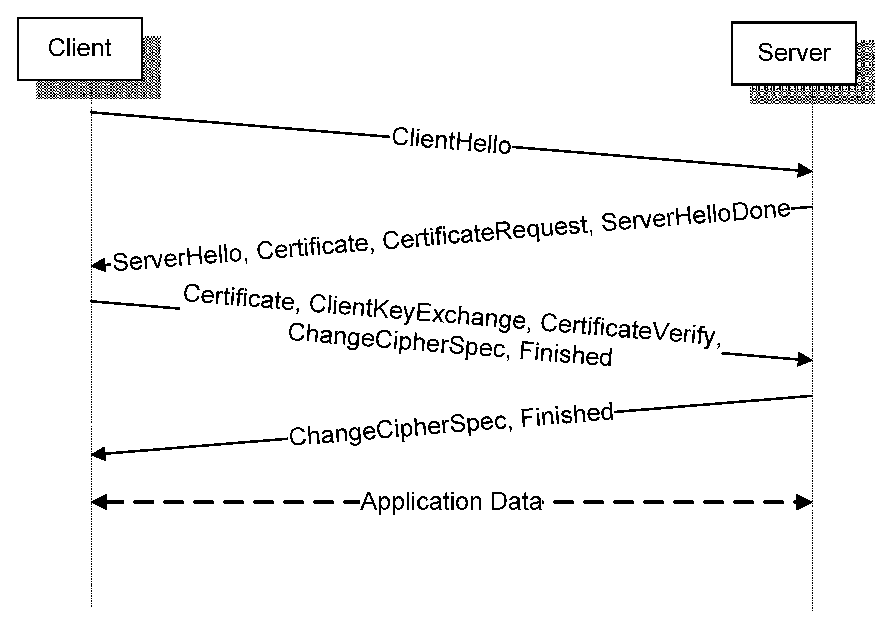
\includegraphics[scale=0.50]{TLS-Client-Authentication}
 \caption{TLS Exchange with Client and Server Authentication.}
 \label{tls-client-authentication-figure}
\end{figure}

\begin{figure}[!t]
 \centering
 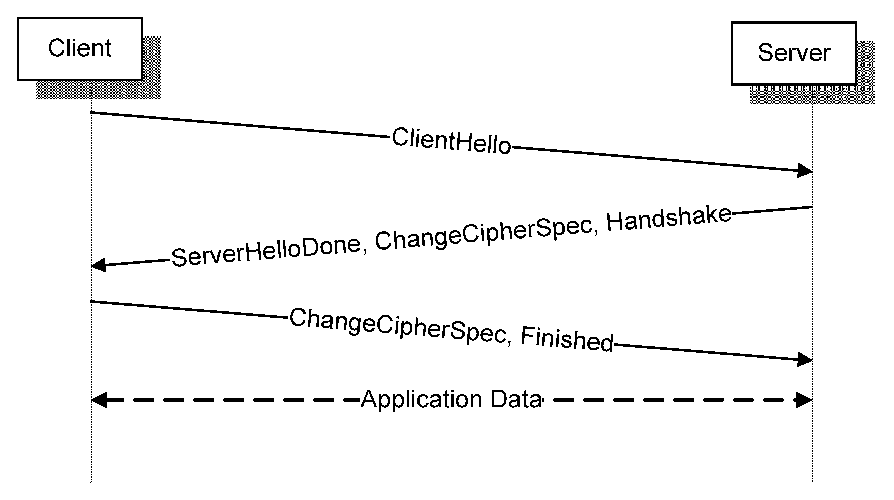
\includegraphics[scale=0.50]{TLS-Session-Resumption}
 \caption{TLS Session Resumption.}
 \label{tls-session-resumption-figure}
\end{figure}

\section{Code Availability}

There are many reasons for reusing protocols developed by the Internet Engineering Task Force (IETF) and one reason relevant to this document is the widespread availability of high-quality open source code. Chances are good that there is already an open source TLS stack available for the smart object hardware platform. In such a case the integration effort is significant lower, which leads to faster time to market and lower development costs. This is not an irrelevant factor in the design of smart objects since costs are not only related to the hardware but also contributed by operating system and application development. 

A compilation of available TLS implementations can be found at \cite{TLS-Implementations}. While many of these implementations provide a good starting point for a developer the axTLS project \cite{axTLS} already claims to offer a small code footprint. Beyond these implementations there is also open source code with EAP-TLS, which is used for network access authentication. Unlike the previous implementations this code first needs to be decoupled from the underlying Extensible Authentication Protocol (EAP) container. The WPA Supplicant \cite{wpa-supplicant} (for the client side) and the FreeRADIUS \cite{FreeRADIUS} (for the server side) contain EAP-TLS libraries that could be utilized -- the WPA Supplicant already provides the support for a small internal crypto library that does not rely on external libraries, like OpenSSL. 

The author had chosen axTLS and the remainder of the paper refers to that specific implementation. axTLS is a C-based implementation of TLS v1.0 and TLS v1.1 and offers the following features: 
\begin{itemize}
\item Certificate support (X509v1, self-signed certificates, PKCS\#8, PKCS\#12 keys/certificates in DER/PEM format), 
\item Certificate verification and identity checks, 
\item Session resumption,
\item Session renegotiation,
\item Various TLS Record Layer cipher algorithms: RC4 with SHA1, AES128 with SHA1, AES256 with SHA1, RC4 with SHA1, RC4 with MD5
\end{itemize}

The axTLS implementation is focused on the support of ciphersuites that use RSA-based key transport and does not support TLS-PSK \cite{rfc4346} or Diffie-Hellman based key exchanges. Digital Signature Algorithm (DSA) and Elliptic Curve Cryptography (ECC) based public key based algorithms are not supported either. 

A useful property of the axTLS implementation is the integration of crypto-libraries. Therefore, no dependencies to external libraries exist.

\section{Communication Relationships}
\label{relationships} 

A security solution is strongly impacted by the communication relationships \cite{rfc4101}, which will have an impact on the code size. Having a good understanding of these relationships will be essential. 

Consider the following scenario where a smart meter transmits its energy readings to other parties. The electricity company will want to make sure that the obtained meter readings can be attributed to a specific meter in a house hold. Most electricity companies will find it unacceptable to have meter readings modified in transit or by a rouge endpoint (particularly if the attack leads to a disadvantage, for example financial loss, for the electricity provider). Users in a house hold may want to ensure that only certain parties get to see the meter readings; privacy concerns come to mind.  

In this example a sensor may need to only ever talk to servers of a specific electricity company or even only to a single pre-configured server\footnote{The server the meter needs to interact with may change over time with the help of software update or configuration changes. These changes to the software of the meter may then also lead to newly provisioned security credentials, such as certificates.} Clearly, some information has to be pre-provisioned into the device to ensure the desired behavior to talk only to selected servers. The meter may be configured with the domain name used by the electricity company and with the root certificate that is used by the electricity company to sign certificates for their servers. The device may, however, also be configured to accept one or multiple server certificates. It may even be pre-provisioned with the server's raw public key, or a shared secret instead of relying on certificates.

Lowering the flexibility decreases the implementation overhead. TLS-PSK \cite{rfc4279}, in case of shared secret usage, or raw public keys used with TLS \cite{I-d.ietf-tls-oob-pubkey} require fewer lines of code than x509 certificate usage, as it will be explained later in this document. A decision for constraining the client-side TLS implementation, for example by offering only a single ciphersuite, has to made in awareness of what functionality will be available on the TLS server-side. In certain communication environments it may be easy to influence both communication partners while in others cases the existing deployment needs to be taken into consideration. 

To illustrate another example, consider an Internet radio who allows a user to connect to available radio stations will be more constrained than an IP-enabled scale that connects only to the Web server offered by the manufacturer of that device. For the Internet radio case a threat assessment may even lead to the conclusion that TLS support is not necessary at all. 

Consider the following extension to our earlier scenario where the meter is attached to a home WLAN network and the interworking with WLAN security mechanisms need to be taken care of. On top of the link layer authentication a transport layer or application layer security mechanism needs to be implemented. Quite likely the security mechanisms will be different due to the different credential requirements. While there is a possibility for re-use of cryptographic libraries (such as the SHA-1, MD5, or HMAC) the overall code footprint will very likely be larger. 

\section{Code Size}

Smart objects are constrained in different ways; flash memory is only one of many constraints. The choice of protocol mechanisms will be impacted by whatever constraint is getting most attention from an engineer. Some design goals are also contradicting with each other. In this paper we focus on code size optimizations. Tradeoffs will have to be made by reducing flexibility and functionality. Consider the following simple example: TLS session resumption leads to an improvement in the initial handshake but requires additional code. The following tables provide information about the code size of various security functions. The code was compiled under Ubuntu Linux using the -Os compiler flag setting for a 64-bit AMD machine. The same environment had been used for all other code compilations in this paper.

\begin{table}[htdp]
\caption{Binary Code Size for Cryptography Support Functions}
\begin{center}
\begin{tabular}{|l|r|}
\hline
\textbf{Library} & \textbf{Code Size}\\
\hline\hline
MD5 & 4,856 bytes \\ 
\hline\hline
SHA1 & 2,432 bytes \\ 
\hline\hline
HMAC & 2,928 bytes \\
\hline\hline
RSA & 3,984 bytes \\
\hline\hline
Big Integer Implementation & 8,328 bytes \\ 
\hline\hline
AES & 7,096 bytes \\
\hline\hline
RC4 & 1,496 bytes \\ 
\hline\hline
Random Number Generator & 4,840 bytes \\
\hline
\end{tabular}
\end{center}
\label{crypto-code-table}
\end{table}

The library implementing the random number generator (RNG) \textit{crypto\_misc.c} allows OS support to be re-used but for the purpose of this illustration it had been disabled and therefore the RNG implementation is purely in software. A hardware platform that provides RNG support may likely lead to a smaller footprint. There are also other support functions that come with \textit{crypto\_misc.c} but those had been excluded with compile-time flags.

\begin{table}[htdp]
\caption{Binary Code Size for TLS-specific Code}
\begin{center}
\begin{tabular}{|p{1cm}|p{0,6cm}|p{5,8cm}|}
\hline
\textbf{Library Name} & \textbf{Code Size} & \textbf{Description} \\
\hline\hline
x509& 2,776 bytes & The x509 related code (\textit{x509.c}) provides functions to parse certificates, to copy them into the program internal data structures and to perform certificate related processing functions, like certificate verification.\\ 
\hline\hline
ASN1 Parser & 5,512 bytes & The ASN1 library (\textit{asn1.c}) contains the necessary code to parse ASN1 data.\\ 
\hline\hline
Generic TLS Library & 15,928 bytes & This library (\textit{tls1.c}) is separated from the TLS client specific code (\textit{tls1\_clnt.c}) to offer those functions that are common with the client and the server-side implementation. This includes code for the master secret generation, certificate validation and identity verification, computing the finished message, ciphersuite related functions, encrypting and decrypting data, sending and receiving TLS messages (e.g., finish message, alert messages, certificate message, session resumption).\\ 
\hline\hline
TLS Client Library & 4,584 bytes & The TLS client-specific code (\textit{tls1\_clnt.c}) includes functions that are only executed by the client based on the supported ciphersuites, such as establishing the connection with the TLS server, sending the ClientHello handshake message, parsing the ServerHello handshake message, processing the ServerHelloDone message, sending the ClientKeyExchange message, processing the CertificateRequest message. \\ 
\hline\hline
OS Wrapper Functions & 2,776 bytes & The functions defined in \textit{os\_port.c} aim to make development easier (e.g., for failure handling with memory allocation and various header definitions) but are not absolutely necessary.\\ 
\hline\hline
OpenSSL Wrapper Functions & 931 bytes & The OpenSSL API calls are familiar to many programmers and therefore these wrapper functions are provided to simplify application development. This library (\textit{openssl.c}) is also not absolutely necessary.\\ 
\hline\hline
Certificate Processing Functions & 4,456 bytes & These functions defined in \textit{loader.c} provide the ability to load certificates from files (or to use a default key as a static data structure embedded during compile time), to parse them, and populate corresponding data structures. \\
\hline
\end{tabular}
\end{center}
\label{tls-code-table}
\end{table}
The code in Table \ref{tls-code-table} includes support for session resumption as well as the necessary functions for certificate validation and identity checking. 

Finally, there is the implementation application that opens a TCP connection to a predefined server address, performs the TLS handshake (with server-side authentication only, RSA encrypted key transport) and establishes the TLS record layer with the RC4-SHA1 ciphersuite. Without the above-mentioned code statically linked to the TLS implementation the object code is 3,816 bytes large. 

%This is certainly a fair amount of code, which will exceed the total amount of flash memory of many devices that are in focus of this discussion, such as an Arduino Uno with it's  32KB of flash memory\footnote{There is Arduino hardware offering more flash memory, such as the Arduino Mega 2560 with 256 KB flash memory, but also more constrained  devices. The current Arduino hardware does not offer hardware crypto support.}.  

To evaluate the required TLS functionality a couple of high level design decisions have to be made:

\begin{enumerate}
\item What type of protection for the data traffic is required? Is confidentiality protection in addition to integrity protection required? Many TLS ciphersuites also provide a variant for NULL encryption. If confidentiality protection is demanded a carefully chosen set of algorithms may have a positive impact on the code size. For example, the RC4 stream cipher code size is 1,496 bytes compared to 7,096 bytes for AES usage. Re-use of crypto-libraries (within TLS but also among the entire protocol stack) will also help to reduce the overall code size. 
\item What functionality is available in hardware? For example, certain hardware platforms offer support for a random number generator as well as cryptographic algorithms (e.g., AES). These functions can be re-used and allow to reduce the amount of required code. 
\item What credentials for client and server authentication are required: passwords, pre-shared secrets, certificates, raw public keys (or a mixture of them)? 
\item What TLS version and what TLS features, such as session resumption, can or have to be used?
\end{enumerate} 

This paper focuses on code size requirements rather than on optimization of RAM, energy consumption, or over-the-wire communication overhead. As detailed in Table \ref{tls-raw-code-table}, the author modified the code of Table \ref{tls-code-table} to provide support for raw public keys, as described in \cite{I-d.ietf-tls-oob-pubkey}. By using \cite{I-d.ietf-tls-oob-pubkey} the TLS client adds an extension of type "cert\_type" to the extended client hello message to indicate support for raw public keys. If the TLS server supports this extension it includes only the SubjectPublicKeyInfo part of the certificate (rather than the entire certificate) in the Certificate message. This leads to a reduction of the data passed over to the client; in our example with the default certificate provided by the axTLS implementation the certificate size was reduced from 475 bytes to 163 bytes (using an RSA-based public key). Note that the SubjectPublicKeyInfo block does not only contain the raw keys, namely the public exponent and the modulus, but also a small ASN1 header preamble.  

Various code optimizations are possible when raw public keys are used instead of certificates. Table \ref{tls-raw-code-table} shows the impact to the code size. 

\begin{table}[htdp]
\caption{Binary Code Size for Raw Key Support in TLS}
\begin{center}
\begin{tabular}{|p{1cm}|p{0,6cm}|p{5,8cm}|}
\hline
\textbf{Library Name} & \textbf{Code Size} & \textbf{Description} \\
\hline\hline
ASN1 Parser & 3,232 bytes & The necessary support from the ASN1 library (\textit{asn1.c}) now only contains functions for parsing of the ASN1 components of the SubjectPublicKeyInfo block.\\ 
\hline\hline
Generic TLS Library & 16,288 bytes & This size of this library (\textit{tls1.c}) was slightly enlarged since additional functionality for loading keys into the bigint data structure, which was previously found in \textit{loader.c} and in \textit{x509.c} is now included in this file. On the other hand, code was removed that relates to certificate processing and functions to retrieve certificate related data (e.g., to fetch the X509 distinguished name or the subject alternative name).\\ 
\hline\hline
TLS Client Library & 4,528 bytes & The TLS client-specific code (\textit{tls1\_clnt.c}) nows contains additional code for the raw public key support, for example in the ClientHello msg. Most functions were left unmodified. \\ 
\hline
\end{tabular}
\end{center}
\label{tls-raw-code-table}
\end{table}

Note that the functionality provided in \textit{loader.c} was reduced to the bare minimum by removing the ability to load different types of certificates from the filesystem. The remaining code was together with the x509 functionality incorporated into \textit{tls1.c}. The author believes that further reductions in code size are accomplishable at the expense of flexibility, protocol performance, and application developer convenience. For example, the code above still offers session resumption support - a feature that consumes a small amount of code space while significantly improving the handshake performance. Also the usage of TLS session resumption without server-side state, see RFC 5077 \cite{rfc5077}, is a reasonable option for devices that communicate infrequently. Code for RFC 5077 is not included in this library.

Of course, the transition to raw public keys does not change the code size of the core crypto functions, such as MD5, SHA-1, and RC4. However, the RSA code size was reduced to 3,544 bytes since the function for decryption is not needed in our setting. 

\section{Conclusion}
TLS is a good example of a wildly\footnote{The IAB published a document, RFC 5218 \cite{rfc5218}, on the success criteria for protocols.  A "wildly successful" protocol far exceeds its original goals, in terms of purpose (being used in scenarios far beyond the initial design), in terms of scale (being deployed on a scale much greater than originally envisaged), or both.} success security protocol that can be tailored to fit the needs of a specific deployment environment. This customization property offers the basis for a relatively small code footprint. The communication model and the security goals will, however, ultimately decide about the resulting code size; this is not only true for TLS but for every security solution. 

More flexibility and more features will translate to a bigger footprint. Generic complains about the large size of TLS stacks are not useful and should be accompanied by a description of the assumed functionality. To support the author's opinion this position paper provides information about the amount of required code for various functions and considers most recent work from the IETF TLS working group for the support of raw public keys\footnote{The author will do further work to reduce the code size (for example by using the new TLS 1.2 PRF) and to cross-compile the code to an ARM-based platform for better comparison with investigations of other teams.}. 

The author is convinced that TLS is a suitable security protocol (with the standardized extensions) for usage in many smart object deployments and only minor extensions, as currently being developed in the IETF TLS working group, are needed to support an even large set of use cases. There are, however, cases where the security goals ask for a security solution other than TLS. With the wide range of smart object applications it is impractical to design for a single security architecture or even a single communication architecture. 

As a next step the author suggests to collect the community experience on TLS about the implementation, system design and deployment decisions that impact the code footprint, size and number of exchanged messages, RAM usage, and energy consumption. This information will be valuable for those working on smart object security. 

\bibliographystyle{IEEEtran}
% \bibliographystyle{acmtrans}
\bibliography{paper}
\end{document}
